\begin{frame}{Sinais analógicos e digitais}
    \begin{columns}[T]
        \begin{column}{0.47\textwidth}
            \begin{block}{Sinal analógico}
                Pode assumir infinitos valores dentro de uma faixa.

                Exemplo: uma tensão entre $0$ V e $3{,}3$ V.
            \end{block}

            \begin{center}
                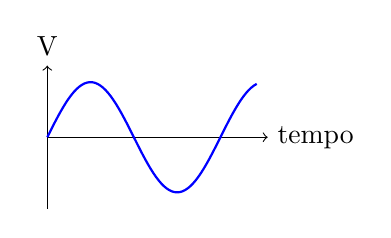
\begin{tikzpicture}[scale=0.7]
                    \draw[->] (0,0) -- (4,0) node[right] {tempo};
                    \draw[->] (0,-1.3) -- (0,1.3) node[above] {V};
                    \draw[blue,thick,domain=0:3.8,samples=80]
                    plot (\x,{sin(2*\x r)});
                \end{tikzpicture}
            \end{center}
        \end{column}

        \begin{column}{0.47\textwidth}
            \begin{block}{Sinal digital}
                Representado por níveis discretos, normalmente 0 e 1.
            \end{block}

            \begin{center}
                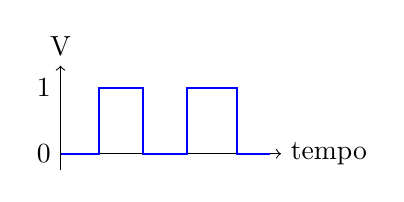
\begin{tikzpicture}[scale=0.7]
                    \draw[->] (0,0) -- (4,0) node[right] {tempo};
                    \draw[->] (0,-0.3) -- (0,1.6) node[above] {V};
                    \draw[blue,thick] (0,0) -- (0.7,0) -- (0.7,1.2)
                    -- (1.5,1.2) -- (1.5,0) -- (2.3,0) -- (2.3,1.2)
                    -- (3.2,1.2) -- (3.2,0) -- (3.8,0);
                    \node[left] at (0,0) {0};
                    \node[left] at (0,1.2) {1};
                \end{tikzpicture}
            \end{center}
        \end{column}
    \end{columns}
\end{frame}